% Asset ID: FA22SimplexAlgorithmTableauTikZ-002
% Unit: FA22 Further A2 2 Applied Mathematics
% Applied section: Section D, Discrete and Decision Mathematics
% Topic code: FA22-ALGGRAPH
% Topic ID: FA22SimplexAlgorithmTableau
% Related LO: FA22-ALGGRAPH-LO003
% Related lesson file: FA22_simplex_algorithm_tableau_lesson.md
% Related lesson section: #9. Visual Asset Integration
% Used placeholder:
% [VISUAL PLACEHOLDER: FA22SimplexAlgorithmTableauTikZ-002 | Source: Uploaded tableau evidence | Insert from tikz/FA22SimplexAlgorithmTableauTikZ-002.tex | Purpose: Provide a clean tableau template that can be reused in examples.]
% Source: Uploaded tableau evidence
% Purpose: Provide a clean tableau template that can be reused in examples.
% Creation status: Generated in Phase 4
% On-spec status: Core CCEA Further Mathematics content, restricted to two-variable linear programming problems.

\documentclass[tikz,border=8pt]{standalone}
\usepackage{amsmath,amssymb}
\usetikzlibrary{arrows.meta,calc,positioning,fit}
\definecolor{Canvas}{HTML}{FAF9F6}
\definecolor{Panel}{HTML}{FFFFF0}
\definecolor{LineSoft}{HTML}{E5E5EA}
\definecolor{Accent}{HTML}{C5A059}
\definecolor{AccentDeep}{HTML}{D4AF37}
\definecolor{TextDark}{HTML}{2C2C2E}
\definecolor{SoftRose}{HTML}{FBEFEF}
\definecolor{SoftGold}{HTML}{FFF7D6}
\begin{document}
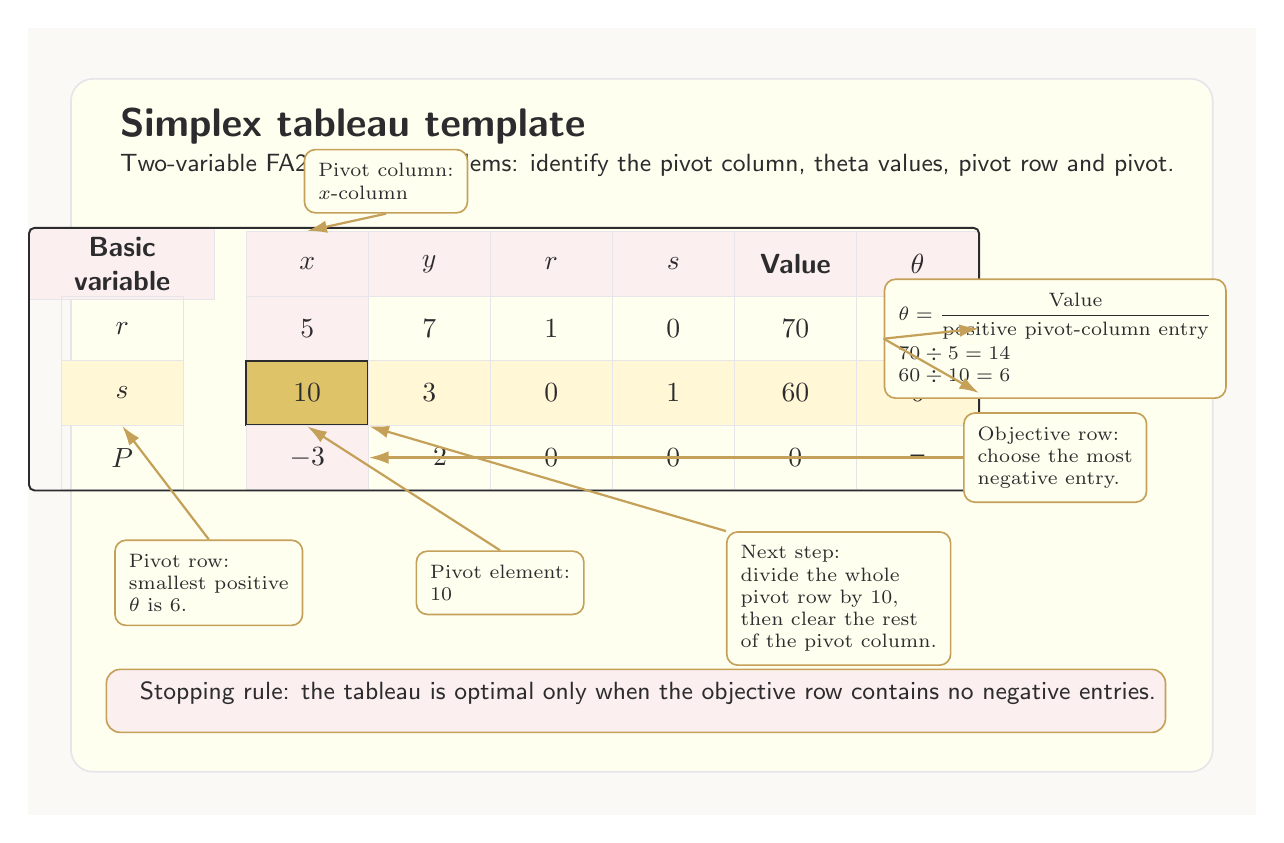
\begin{tikzpicture}[every node/.style={font=\sffamily,text=TextDark},cell/.style={draw=LineSoft,line width=0.45pt,minimum width=1.55cm,minimum height=0.82cm,align=center},head/.style={cell,fill=SoftRose,font=\sffamily\bfseries},sidehead/.style={cell,fill=SoftRose,font=\sffamily\bfseries,minimum width=2.35cm},pivotcol/.style={fill=SoftRose},pivotrow/.style={fill=SoftGold},pivotcell/.style={fill=AccentDeep!75,draw=TextDark,line width=0.7pt},note/.style={draw=Accent,fill=Panel,rounded corners=4pt,line width=0.6pt,align=left,inner sep=5pt,font=\scriptsize},arrow/.style={draw=Accent,line width=0.8pt,-{Latex[length=2.5mm,width=1.6mm]}}]
\fill[Canvas] (-1.2,-5.0) rectangle (14.4,5.0); \filldraw[fill=Panel,draw=LineSoft,line width=0.6pt,rounded corners=8pt](-0.65,-4.45) rectangle (13.85,4.35);
\node[anchor=west,font=\sffamily\bfseries\Large] at (-0.15,3.75){Simplex tableau template};
\node[anchor=west,font=\sffamily\small] at (-0.15,3.25){Two-variable FA22 simplex problems: identify the pivot column, theta values, pivot row and pivot.};
\node[sidehead](h0) at (0,2){Basic\\variable};\node[head,pivotcol](h1) at (2.35,2){$x$};\node[head](h2) at (3.90,2){$y$};\node[head](h3) at (5.45,2){$r$};\node[head](h4) at (7.00,2){$s$};\node[head](h5) at (8.55,2){Value};\node[head](h6) at (10.10,2){$\theta$};
\node[cell](r10) at (0,1.18){$r$};\node[cell,pivotcol](r11) at (2.35,1.18){$5$};\node[cell](r12) at (3.90,1.18){$7$};\node[cell](r13) at (5.45,1.18){$1$};\node[cell](r14) at (7.00,1.18){$0$};\node[cell](r15) at (8.55,1.18){$70$};\node[cell](r16) at (10.10,1.18){$14$};
\node[cell,pivotrow](r20) at (0,0.36){$s$};\node[cell,pivotrow,pivotcol,pivotcell](r21) at (2.35,0.36){$10$};\node[cell,pivotrow](r22) at (3.90,0.36){$3$};\node[cell,pivotrow](r23) at (5.45,0.36){$0$};\node[cell,pivotrow](r24) at (7.00,0.36){$1$};\node[cell,pivotrow](r25) at (8.55,0.36){$60$};\node[cell,pivotrow](r26) at (10.10,0.36){$6$};
\node[cell](r30) at (0,-0.46){$P$};\node[cell,pivotcol](r31) at (2.35,-0.46){$-3$};\node[cell](r32) at (3.90,-0.46){$-2$};\node[cell](r33) at (5.45,-0.46){$0$};\node[cell](r34) at (7.00,-0.46){$0$};\node[cell](r35) at (8.55,-0.46){$0$};\node[cell](r36) at (10.10,-0.46){--};
\node[draw=TextDark,line width=0.7pt,rounded corners=2pt,inner sep=0pt,fit=(h0)(h6)(r30)(r36)]{};
\node[note](objnote) at (11.85,-0.46){Objective row:\\choose the most\\negative entry.};\draw[arrow](objnote.west)--(r31.east);
\node[note](pcnote) at (3.35,3.05){Pivot column:\\$x$-column};\draw[arrow](pcnote.south)--(h1.north);
\node[note](trnote) at (11.85,1.05){$\theta=\dfrac{\text{Value}}{\text{positive pivot-column entry}}$\\[2pt]$70\div5=14$\\$60\div10=6$};\draw[arrow](trnote.west)--(r16.east);\draw[arrow](trnote.west)--(r26.east);
\node[note](prnote) at (1.1,-2.05){Pivot row:\\smallest positive\\$\theta$ is $6$.};\draw[arrow](prnote.north)--(r20.south);
\node[note](pnote) at (4.8,-2.05){Pivot element:\\$10$};\draw[arrow](pnote.north)--(r21.south);
\node[note](rownote) at (9.1,-2.25){Next step:\\divide the whole\\pivot row by $10$,\\then clear the rest\\of the pivot column.};\draw[arrow](rownote.north west)--(r21.south east);
\filldraw[fill=SoftRose,draw=Accent,line width=0.6pt,rounded corners=5pt](-0.2,-3.95) rectangle (13.25,-3.15);
\node[anchor=west,font=\sffamily\small] at (0.1,-3.45){Stopping rule: the tableau is optimal only when the objective row contains no negative entries.};
\end{tikzpicture}
\end{document}
